\FloatBarrier
\section{Arquitetura de Controle de Movimento (Vis\~ao Geral)}
\label{sec:ctrl-visao-geral}

O subsistema de movimento foi dividido em dois la\c{c}os temporizados:
(i) \textbf{TIM6} a \SI{50}{kHz} (\SI{20}{\micro\second} por tick), dedicado \`a gera\c{c}\~ao de pulsos \emph{STEP} a partir de um DDA (Digital Differential Analyzer) em ponto fixo; e
(ii) \textbf{TIM7} a \SI{1}{kHz} (\SI{1}{ms}), dedicado \`a l\'ogica de rampa trapezoidal (acelera\c{c}\~ao/desacelera\c{c}\~ao), ajuste de velocidade efetiva, leitura dos encoders e controle PI de posi\c{c}\~ao.
A separa\c{c}\~ao reduz jitter na largura do \emph{STEP} e garante que o c\'alculo das rampas e do PI n\~ao impacte o \emph{timing} do pulso. As constantes de tempo usadas no c\'odigo s\~ao:
\texttt{MOTION\_TIM6\_HZ=50000}, \texttt{MOTION\_STEP\_HIGH\_TICKS=1}, \texttt{MOTION\_STEP\_LOW\_TICKS=1}, \texttt{MOTION\_DIR\_SETUP\_TICKS=1}, \texttt{MOTION\_ENABLE\_SETTLE\_TICKS=2}.

\subsection{Compatibilidade de \emph{timing} com o TMC5160 (\emph{STEP}/\emph{DIR})}
\label{subsec:tmc-step-dir}

De acordo com o datasheet do TMC5160, as entradas \emph{STEP} e \emph{DIR} possuem filtragem anal\'ogica ($t_{\text{FILTSD}}\approx\SI{20}{ns}$) e requerem tempos m\'inimos:
$t_{SH}$ (alto de STEP) e $t_{SL}$ (baixo de STEP) $\ge \max(t_{\text{FILTSD}},\,t_{\text{CLK}}+20\text{ ns})$ (tipicamente $\ge\SI{100}{ns}$). Os tempos de \emph{setup/hold} s\~ao $t_{DSU}=\SI{20}{ns}$ (DIR antes de STEP) e $t_{DSH}=\SI{20}{ns}$ (DIR ap\'os STEP) \cite{tmc5160_ds}.
No nosso projeto, com \textbf{TIM6 a 50 kHz}, configuramos \emph{guardas} muito acima do m\'inimo (margem de seguran\c{c}a):
\begin{itemize}
  \item Largura alta de STEP: $t_{SH} = \texttt{MOTION\_STEP\_HIGH\_TICKS}\cdot\SI{20}{\micro s} = \SI{20}{\micro s}$;
  \item Tempo baixo entre pulsos: $t_{SL} = \texttt{MOTION\_STEP\_LOW\_TICKS}\cdot\SI{20}{\micro s} = \SI{20}{\micro s}$;
  \item \emph{Setup} de DIR: $t_{DSU} = \texttt{MOTION\_DIR\_SETUP\_TICKS}\cdot\SI{20}{\micro s} = \SI{20}{\micro s}$;
  \item \emph{Settle} de ENABLE: $\texttt{MOTION\_ENABLE\_SETTLE\_TICKS}\cdot\SI{20}{\micro s} = \SI{40}{\micro s}$.
\end{itemize}

\begin{figure}[H]
    \centering
    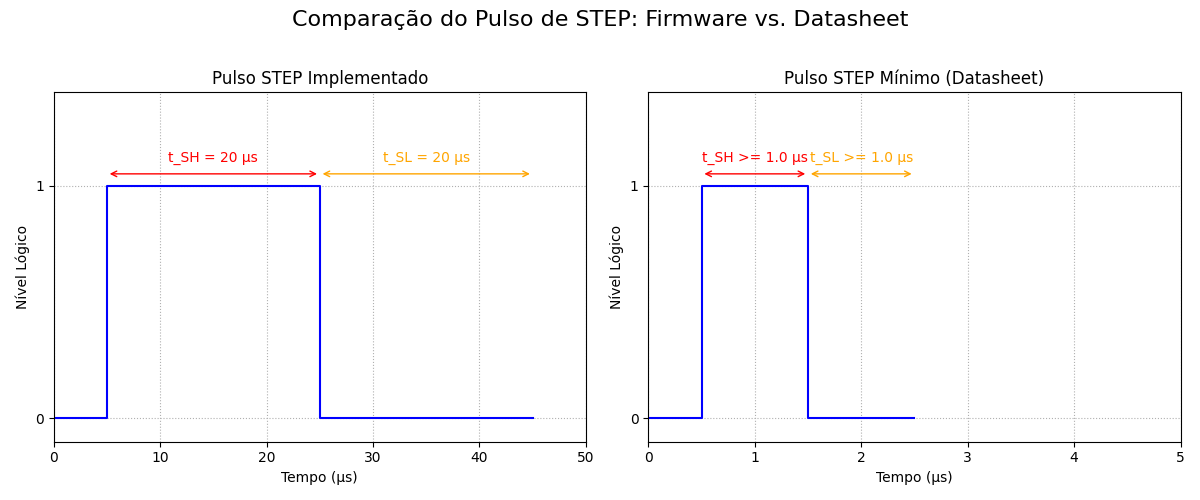
\includegraphics[width=\textwidth]{Cap03/step_pulse_comparison.png}
    \caption{Compara\c{c}\~ao visual entre o pulso de STEP implementado no firmware (esquerda) e o pulso m\'inimo requerido pelo datasheet do TMC5160 (direita), evidenciando a robusta margem de tempo utilizada.}
    \label{fig:step_pulse_comparison}
\end{figure}
Logo, todos os requisitos do TMC5160 s\~ao amplamente atendidos com folga (vide Tabela~\ref{tab:tmc-timing-vs-projeto}).

\begin{table}[H]
  \centering
  \caption{Tempos de STEP/DIR: TMC5160 (datasheet) vs. implementa\c{c}\~ao.}
  \label{tab:tmc-timing-vs-projeto}
  \setlength{\tabcolsep}{4pt}\footnotesize
  \begin{tabularx}{\textwidth}{lcccX}
    \toprule
    Par\^ametro & TMC5160 (m\'in.) & Projeto & Margem & Observa\c{c}\~ao \\
    \midrule
    $t_{SH}$ (alto de STEP) & $\ge \max(t_{\text{FILTSD}}, t_{\text{CLK}}+20\text{ ns})$ ($\gtrsim \SI{100}{ns}$) & \SI{20}{\micro s} & $\times 200{,}000$ & \texttt{MOTION\_STEP\_HIGH\_TICKS}=1 \\
    $t_{SL}$ (baixo de STEP) & idem & \SI{20}{\micro s} & $\times 200{,}000$ & \texttt{MOTION\_STEP\_LOW\_TICKS}=1 \\
    $t_{DSU}$ (DIR\,$\rightarrow$\,STEP) & \SI{20}{ns} & \SI{20}{\micro s} & $\times 1{,}000$ & \texttt{MOTION\_DIR\_SETUP\_TICKS}=1 \\
    $t_{DSH}$ (STEP\,$\rightarrow$\,DIR) & \SI{20}{ns} & \SI{20}{\micro s} & $\times 1{,}000$ & Garantido pelo espa\c{c}amento de pulsos \\
    ENABLE settle & n.\,d. (com filtro interno) & \SI{40}{\micro s} & -- & \texttt{MOTION\_ENABLE\_SETTLE\_TICKS}=2 \\
    \bottomrule
  \end{tabularx}
\end{table}

\noindent
Com $t_{SH}=t_{SL}=\SI{20}{\micro s}$, o per\'iodo m\'inimo de STEP \'e $\SI{40}{\micro s}$ e a frequ\^encia m\'axima f\'isica por eixo fica:
\[
\texttt{MOTION\_MAX\_SPS} \;=\; 
\frac{\texttt{MOTION\_TIM6\_HZ}}{\texttt{MOTION\_STEP\_HIGH\_TICKS}+\texttt{MOTION\_MIN\_LOW\_TICKS}}
\;=\; \frac{50\,000}{1+1} \;=\; \SI{25}{kSPS}.
\]

\subsection{MicroPlyer, resolu\c{c}\~ao e DEDGE}
Quando \texttt{intpol}=1 em \texttt{CHOPCONF}, o TMC5160 interpola cada pulso de STEP at\'e 256 microsteps (\emph{MicroPlyer}), melhorando suavidade a partir de entradas com resolu\c{c}\~ao mais grossa. O bit \texttt{dedge} define se as duas bordas do STEP contam (requer duty de 50\%) ou apenas a borda de subida. No nosso sistema, os pulsos t\^em duty controlado e largura fixa, e a contagem por borda de subida (padr\~ao) j\'a atende estabilidade e evita assimetria. Veja \cite{tmc5160_ds} para detalhes.

\FloatBarrier
\section{DDA em Ponto Fixo (TIM6 @ 50\,kHz)}
\label{sec:dda}

A Figura~\ref{fig:firmware_dda_sim} ilustra o funcionamento interno do DDA para um movimento de 7 passos em X e 4 em Y, conforme implementado no firmware. A cada tick do temporizador (eixo horizontal), os acumuladores de fase de X e Y s\~ao incrementados por valores fixos, proporcionais \`as suas respectivas velocidades. O eixo X, sendo mais r\'apido para este vetor, tem um incremento maior e seu acumulador transborda (\emph{overflow}) mais frequentemente. Cada transbordamento, marcado pela volta do acumulador a zero no gr\'afico superior, corresponde \`a gera\c{c}\~ao de um pulso STEP para o eixo, como visto no gr\'afico inferior. Ao final do processo, 7 pulsos foram gerados para X e 4 para Y, distribu\'idos no tempo de forma a manter a trajet\'oria da reta definida pelo host.

\begin{figure}[H]
    \centering
    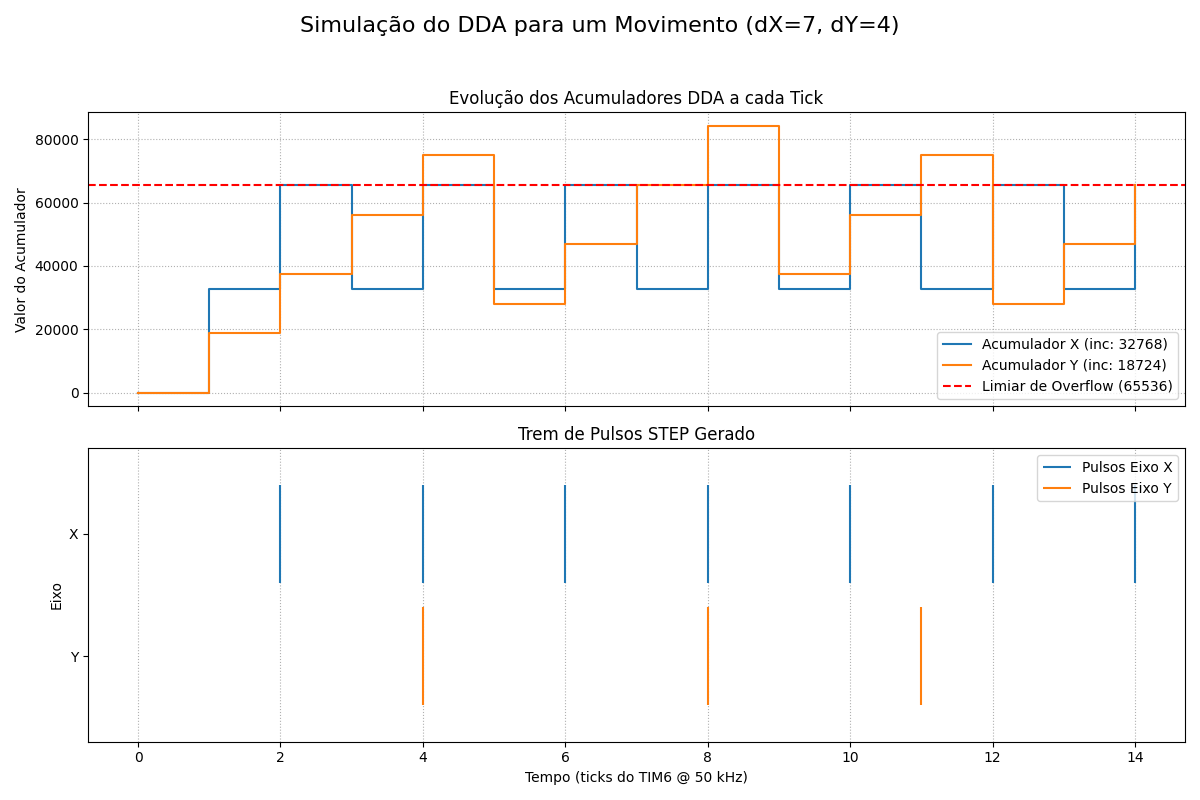
\includegraphics[width=\textwidth]{Cap03/firmware_dda_simulation.png}
    \caption{Simula\c{c}\~ao da opera\c{c}\~ao interna do DDA para um movimento de 7 passos em X e 4 em Y. O gr\'afico superior mostra a evolu\c{c}\~ao dos acumuladores de fase, e o inferior mostra os pulsos STEP gerados para cada eixo a cada transbordamento.}
    \label{fig:firmware_dda_sim}
\end{figure}

O gerador de passos usa um DDA Q16.16. Para cada eixo $i$, mantemos:
\begin{itemize}
  \item acumulador \texttt{dda\_accum\_q16} e incremento \texttt{dda\_inc\_q16};
  \item velocidade efetiva \texttt{v\_actual\_sps} (steps/s), atualizada no TIM7;
  \item contadores de largura do STEP: \texttt{step\_high} e \texttt{step\_low}.
\end{itemize}
A cada tick do TIM6 (\SI{20}{\micro s}):
\[
\texttt{dda\_accum\_q16} \leftarrow \texttt{dda\_accum\_q16} + \texttt{dda\_inc\_q16}.
\]
Quando \texttt{dda\_accum\_q16} $\ge 1.0$ (i.e., \texttt{Q16\_1}), emitimos um pulso de STEP:
\[
\texttt{step\_high} \leftarrow \texttt{MOTION\_STEP\_HIGH\_TICKS},\qquad
\texttt{emitted\_steps} \leftarrow \texttt{emitted\_steps}+1,
\]
baixando o pino ao final de \texttt{step\_high} e respeitando \texttt{step\_low} (t$_{SL}$).
O incremento \'e derivado da velocidade efetiva:
\[
\texttt{dda\_inc\_q16} \;=\; \mathrm{Q16}\!\left(\frac{\texttt{v\_actual\_sps}}{\texttt{MOTION\_TIM6\_HZ}}\right).
\]
Essa rela\c{c}\~ao garante linearidade entre \emph{steps/s} e a taxa de \emph{crossing} do DDA, com jitter sub-\SI{}{\micro s} e duty fixo (ver fun\c{c}\~ao \texttt{motion\_on\_tim6\_tick}).

\FloatBarrier
\section{Rampa Trapezoidal (TIM7 @ 1\,kHz)}
\label{sec:rampa}

A cada \SI{1}{ms}, o TIM7 atualiza a velocidade alvo e aplica a rampa:
\begin{align*}
  \texttt{v\_cmd\_sps} &= \texttt{velocity\_per\_tick}\times 1000, \\
  s_{\text{brake}} &= \left\lfloor \frac{v^2}{2a} \right\rfloor, \quad v=\texttt{v\_actual\_sps},\; a=\texttt{accel\_sps2},
\end{align*}
onde $s_{\text{brake}}$ decide o instante de iniciar a desacelera\c{c}\~ao.
A acelera\c{c}\~ao discreta usa um acumulador de \SI{1}{ms} (\texttt{g\_v\_accum}) para integrar $a$ em passos unit\'arios de velocidade. A l\'ogica segue:
\begin{enumerate}
  \item Se $\text{passos remanescentes} \le s_{\text{brake}}$, reduza $v$ (freio).
  \item Caso contr\'ario, ajuste $v$ gradualmente at\'e $\texttt{v\_cmd\_sps}$, sem ultrapassar \texttt{MOTION\_MAX\_SPS}.
  \item Compute \texttt{dda\_inc\_q16} a partir de \texttt{v\_actual\_sps} (Eq. anterior).
\end{enumerate}
O projeto mant\'em \texttt{DEMO\_ACCEL\_SPS2=\num{200000}} como acelera\c{c}\~ao padr\~ao (substitu\'ivel por eixo). A fun\c{c}\~ao \texttt{motion\_remaining\_steps\_total\_for\_axis} soma segmento ativo + fila para desacelera\c{c}\~ao suave entre trechos.

\begin{figure}[H]
  \centering
  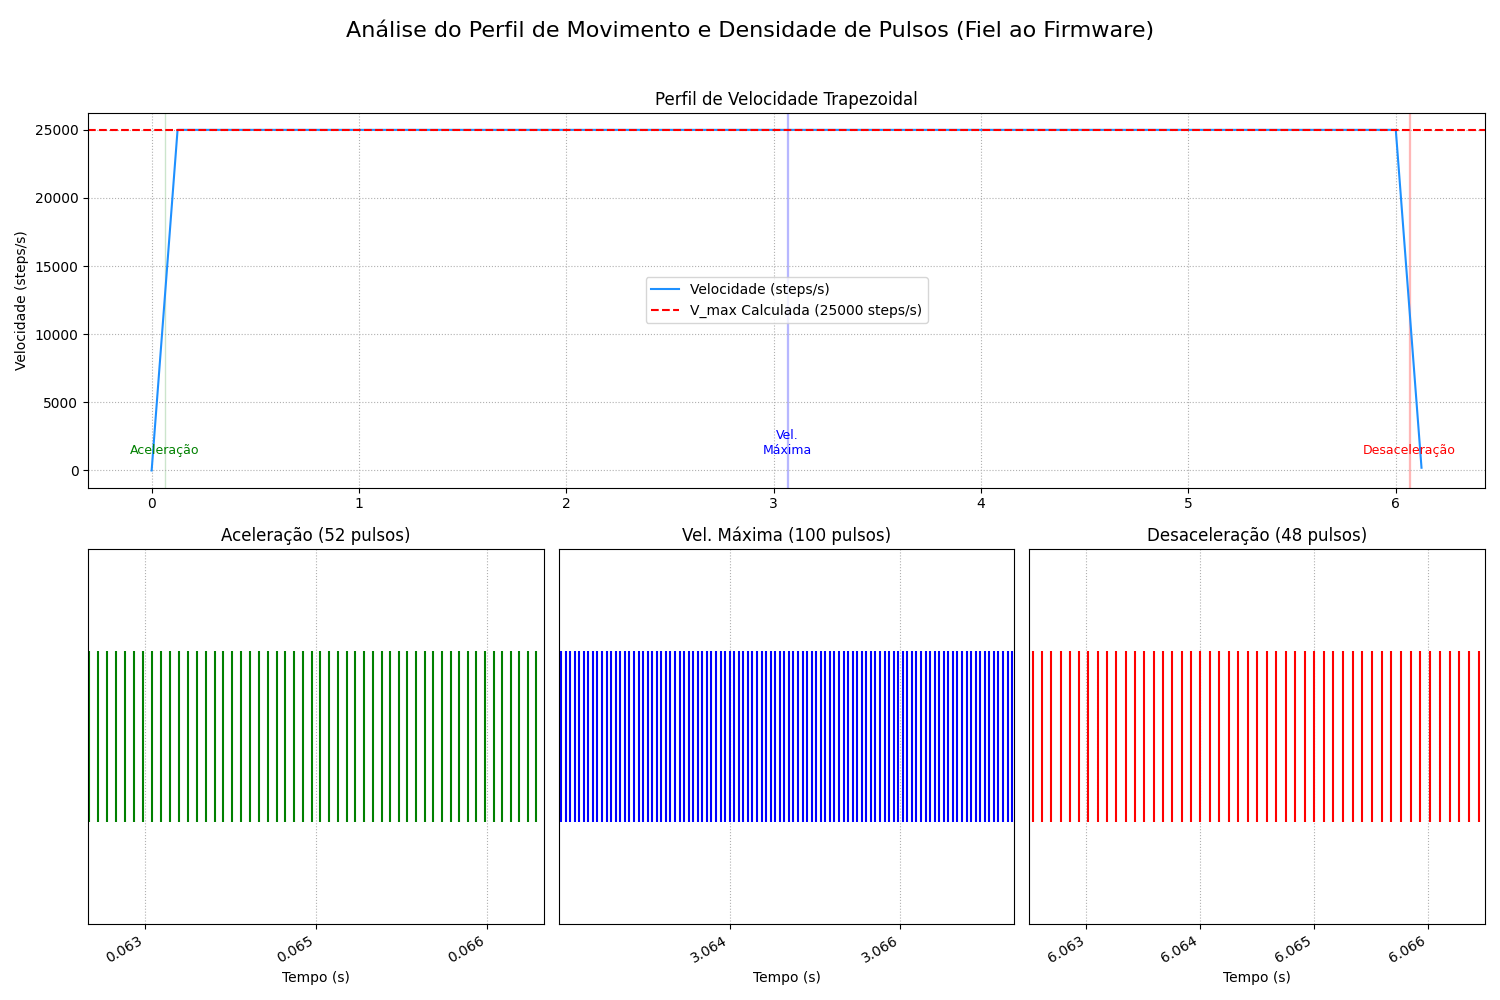
\includegraphics[width=0.8\textwidth]{Cap03/rampa_trapezoidal.png}
  \caption{Perfil de velocidade da rampa trapezoidal simulado a partir dos parâmetros do firmware.}
  \label{fig:rampa_trapezoidal_simulada}
\end{figure}

\FloatBarrier
\section{Controle PI de Posi\c{c}\~ao com Encoder}
\label{sec:pi}

O erro posicional em \emph{passos DDA} \'e
\[
e = \texttt{target\_steps} - \left\lfloor \frac{(\texttt{enc\_rel})\cdot \texttt{DDA\_STEPS\_PER\_REV}}{\texttt{ENC\_COUNTS\_PER\_REV}} \right\rfloor,
\]
com \texttt{DDA\_STEPS\_PER\_REV} $= 400 \times \texttt{MICROSTEP\_FACTOR}$ (passo do motor \SI{0,9}{\degree}) e
\texttt{ENC\_COUNTS\_PER\_REV} por eixo ($X/Z=\num{40000}$, $Y=\num{2500}$).
Aplica-se \emph{deadband} de $\pm$\,\texttt{MOTION\_PI\_DEADBAND\_STEPS} e um filtro exponencial na derivada:
\[
d[n] \leftarrow d[n-1] + \frac{\Delta e - d[n-1]}{2^{\alpha}},\quad \alpha=8.
\]
Os ganhos \texttt{kp}, \texttt{ki}, \texttt{kd} s\~ao inteiros de 16\,bits; a sa\'ida (em \emph{steps/s}) \'e escalada por $2^{-8}$:
\[
\Delta v = \frac{k_p\,e + k_i \sum e + k_d\,d}{2^{8}},
\]
com \emph{anti-windup} (clamp da integral em $\pm\,$\texttt{MOTION\_PI\_I\_CLAMP}) e satura\c{c}\~ao sim\'etrica em $\pm\,$\texttt{MOTION\_MAX\_SPS}. A corre\c{c}\~ao ajusta \texttt{v\_cmd\_sps} antes da rampa, preservando limites f\'isicos (\S\ref{sec:rampa}).

\FloatBarrier
\section{Fila de Movimentos e Segmenta\c{c}\~ao}
\label{sec:fila}

O protocolo host enfileira segmentos (\texttt{move\_queue\_add}) com \texttt{S=(sx,sy,sz)} e velocidade base \texttt{V=(vx,vy,vz)}.
No in\'icio de cada trecho (\texttt{motion\_begin\_segment\_locked}), o c\'odigo:
(1) zera acumuladores do DDA; (2) aplica guardas de ENABLE e DIR; (3) inicializa \texttt{v\_target\_sps} por eixo; e
(4) habilita sa\'ida (\texttt{motion\_hw\_enable}) apenas se \texttt{total\_steps>0}.
A transi\c{c}\~ao para o pr\'oximo segmento acontece quando todos os eixos terminam (\texttt{emitted\_steps==total\_steps}) e nenhum pulso est\'a alto.

\FloatBarrier
\section{Mapeamento para o TMC5160}
\label{sec:tmc-mapeamento}

\subsection{Gera\c{c}\~ao de STEP/DIR (\emph{``PWM'' de passo})}
O driver TMC5160 em modo \emph{STEP/DIR} espera pulsos compat\'iveis com os tempos da Tabela~\ref{tab:tmc-timing-vs-projeto}. O nosso \emph{backend} de GPIO (\texttt{motion\_hw\_*}) implementa:
\begin{enumerate}
  \item \textbf{Largura de STEP} fixa, via \texttt{step\_high} (\SI{20}{\micro s}), garantindo $t_{SH}$.
  \item \textbf{Baixo m\'inimo} via \texttt{step\_low} (\SI{20}{\micro s}), garantindo $t_{SL}$.
  \item \textbf{Setup de DIR} antes do primeiro STEP do trecho, via \texttt{dir\_settle\_ticks}=\SI{20}{\micro s}.
  \item \textbf{ENABLE settle} (\SI{40}{\micro s}) antes de iniciar emiss\~ao.
\end{enumerate}
Com isso, o sinal \emph{STEP} tem duty $\approx$50\% em regime (1~tick alto, 1~tick baixo), o que tamb\'em \'e adequado caso \texttt{dedge}=1 (duas bordas) \cite{tmc5160_ds}.

\subsection{Resolu\c{c}\~ao de microstepping e MicroPlyer}
O host pode ajustar \texttt{MICROSTEP\_FACTOR} em tempo de parada via comando \texttt{set\_microsteps}. Quando \texttt{intpol}=1 no TMC5160, a resolu\c{c}\~ao efetiva de corrente/torque nas bobinas pode ser maior do que a resolu\c{c}\~ao de STEP, garantindo suavidade (Se\c{c}\~ao 15.3, \emph{MicroPlyer}) \cite{tmc5160_ds}.

\FloatBarrier
\section{Par\^ametros-chaves do Projeto}
\label{sec:parametros}

\begin{table}[H]
  \centering
  \caption{Par\^ametros de tempo e limites usados no firmware.}
  \label{tab:param}
  \setlength{\tabcolsep}{4pt}\footnotesize
  \begin{tabularx}{\textwidth}{lXl}
    \toprule
    Par\^ametro & Significado & Valor p/ testes \\
    \midrule
    \texttt{MOTION\_TIM6\_HZ} & Frequ\^encia do la\c{c}o de DDA/STEP & \SI{50}{kHz} \\
    \texttt{MOTION\_STEP\_HIGH\_TICKS} & Largura alta do STEP (m\'in.) & 1 tick = \SI{20}{\micro s} \\
    \texttt{MOTION\_STEP\_LOW\_TICKS} & Baixo m\'inimo entre pulsos & 1 tick = \SI{20}{\micro s} \\
    \texttt{MOTION\_DIR\_SETUP\_TICKS} & \emph{Setup} de DIR antes do STEP & 1 tick = \SI{20}{\micro s} \\
    \texttt{MOTION\_ENABLE\_SETTLE\_TICKS} & \emph{Settle} ap\'os ENABLE & 2 ticks = \SI{40}{\micro s} \\
    \texttt{MOTION\_MAX\_SPS} & Limite f\'isico de \emph{steps/s} & \SI{25}{kSPS} \\
    \texttt{DEMO\_ACCEL\_SPS2} & Acelera\c{c}\~ao padr\~ao & \num{200000} \,steps/s$^{2}$ \\
    \texttt{MOTION\_PI\_DEADBAND\_STEPS} & Zona morta do PI (posi\c{c}\~ao) & 1 passo \\
    \texttt{MOTION\_PI\_I\_CLAMP} & \emph{Anti-windup} da integral & $\pm\,200\,000$ \\
    \bottomrule
  \end{tabularx}
\end{table}

\FloatBarrier
\section{Boas pr\'aticas e Diagn\'ostico}
\label{sec:boaspraticas}

\begin{itemize}
  \item \textbf{Ordem dos eventos}: ajustar DIR $\rightarrow$ respeitar \texttt{dir\_settle\_ticks} $\rightarrow$ habilitar driver $\rightarrow$ respeitar \texttt{en\_settle\_ticks} $\rightarrow$ iniciar STEP.
  \item \textbf{Jitter baixo no STEP}: manter o trabalho pesado (PI, rampa, telemetria) no TIM7; evitar \texttt{printf} em interrup\c{c}\~oes do TIM6 (\texttt{MOTION\_DEBUG\_TIM6\_PRINTS}=0).
  \item \textbf{Telemetria}: \texttt{encoder\_status} e \texttt{set\_origin} exp\~oem posi\c{c}\~ao absoluta/relativa, erro do PI e refer\^encia do zero.
  \item \textbf{Compatibilidade com o TMC5160}: manter $t_{SH}$, $t_{SL}$, $t_{DSU}$ e $t_{DSH}$ com folga; se usar \texttt{dedge}=1, garantir duty de 50\% e bordas limpas (\cite{tmc5160_ds}).
\end{itemize}

\FloatBarrier
\section{Refer\^encias cruzadas}
\label{sec:refs-cruzadas}

Para temporizadores e modos de encoder do STM32L4, ver \cite{stm32l4_rm}. Para o modo \emph{STEP/DIR}, \emph{MicroPlyer} e \emph{timing} do TMC5160, ver \cite{tmc5160_ds}.
